\documentclass{beamer}
\beamertemplatenavigationsymbolsempty
\usecolortheme{beaver}
\setbeamertemplate{blocks}[rounded=true, shadow=true]
\setbeamertemplate{footline}[page number]
%
\usepackage[utf8]{inputenc}
\usepackage[english,russian]{babel}
\usepackage{amssymb,amsfonts,amsmath,mathtext}
\usepackage{subfig}
\usepackage[all]{xy} % xy package for diagrams
\usepackage{array}
\usepackage{multicol} % many columns in slide
\usepackage{hyperref} % urls
\usepackage{hhline} %tables
\usepackage{comment} %comments
% Your figures are here:
\graphicspath{ {fig/} {../fig/} }
\usepackage{sepfootnotes}
\DeclareMathOperator\supp{supp}
\usepackage{tikz}
\usepackage{lmodern}
\newtheorem{theorem}{Теорема}
\newtheorem*{theorem-non}{Теорема}
\usepackage[font=tiny,labelfont=bf]{caption}
%...
%----------------------------------------------------------------------------------------------------------

\title[\hbox to 56mm{Многократное обучение}]{Вырождение распределений при  многократном  \\ обучении в рекомендательных системах}
\author[Н.\,А.~Крехов]{Николай Александрович Крехов}
\institute{Московский физико-технический институт}
\date{\footnotesize
\par\smallskip\emph{Курс:} Моя первая научная статья
\par\smallskip\emph{Эксперт:} к.ф.-м.н. А.\,С.~Хританков
\par\smallskip\emph{Консультант:} А.\,С.~Веприков
\par\bigskip\small 2024}

%----------------------------------------------------------------------------------------------------------

\begin{document}

%----------------------------------------------------------------------------------------------------------

\begin{frame}

    \thispagestyle{empty}
    \maketitle
    
\end{frame}

%-----------------------------------------------------------------------------------------------------

\begin{frame}{Цель исследования}

Мы рассматриваем системы рекомендации товаров пользователям. Изучаем поведение таких системы во времени. Наша задача состоит в том, чтобы развить результат полученный в статье [1] с учетом эффектов feedback loops [2] и filter bubbles [3].
    \begin{block}{Цель}
        Исследование изменений распределений пользователей и товаров в динамической системе с рекомендательным алгоритмом.
    \end{block}
    \begin{block}{Задача}
        Предложить алгоритм, который повышает качество рекомендаций при условии, что не происходит вырождения(т.е. снижения разнообразия) товаров и пользователей.
    \end{block}

\end{frame}

%-----------------------------------------------------------------------------------------------------

% \begin{frame}{Алгоритм рекомендации}



% \item  \footnotesize Сделка: $y_{c,w} \sim Bern(u_{\text{true}}(c, w, z))$

% \item Рассматриваем класс рекомендательных алгоритмов, которые оценивают $u_{\text{true}}(c, w, z)$ через $u_{\text{pred}}(c, w)$

% \begin{columns}[c]

%     \column{0.55\textwidth}
%     Рекомендательный алгоритм:
%         \begin{enumerate}
%             \item Вычисляет функцию $u_{\text{pred}}(c, w)$ для всех $c,\ w$
%             \item Для каждого $c$ по функци $u_{\text{pred}}$ выбирает множество товаров размера $k$ для рекомендации: $\{w_{i_1},\ldots, w_{i_k}\}$
%         \end{enumerate}
    
%     \column{0.60\textwidth}
%         \begin{tikzpicture}
%             \node[draw, rectangle] (customer) at (0,0) {Customer $(c^{d_1},\ldots,c^{d_c})^T$};
%             \node[draw, circle, text width=2cm] (item1) at (-2,-3) {Item 1  $(w_1^{d_1},\ldots,w_1^{d_w})^T$};
%             \node[draw, circle, text width=2cm] (item2) at (2,-3) {Item 2 $(w_2^{d_1},\ldots,w_2^{d_w})^T$};
            
%             \draw[->, green] (customer.200) to[out=-135,in=90] node[midway, above, sloped] {\scriptsize $y_{c, w^1} = 1$} (item1);
%             \draw[->] (item1.45) to[out=45,in=-45] (customer.200);
    
            
%             \draw[->, red] (customer.-20) to[out=-135,in=135] node[midway, above, sloped] {\scriptsize$y_{c, w^2} = 0$} (item2);
%             \draw[->] (item2.90) to[out=45,in=-45] (customer.-20);
    
%         \end{tikzpicture}

% \end{columns}
% Примеры алгоритмов:

%     \begin{itemize}
%         \item[-] TopPopularity
%         \item[-] Random
%         \item[-] Collaborative Filtering using SVD
%     \end{itemize}    
    
% \end{frame}

%-----------------------------------------------------------------------------------------------------


\begin{frame}{Математическая постановка задачи}
 \scriptsize{Пользователи  и товары: $C \subset \mathbb{R}^d, W \subset \mathbb{R}^l$. На каждом шаге $t$ имеется совместное распределение: $(c, w)^T \sim p^{t}_{c,w} (x_c , x_w )$
 
 % $u^t_{\text{true}}: \mathbb{R}^{d_c} \times \mathbb{R}^{d_w} \times \Omega_z \to [0; 1]$ - функция полезности товара для данного пользователя.}
 % \\
\item
Предполгаем, что существует функция $u_{\text{true}}(c, w, z)$, которая показывает вероятность совершения сделки. \\
Рассмтриваемый класс рекомендательных алгоримтов: 
\begin{enumerate}
    \item Cтроит функцию  $u^t_{\text{pred}}(c, w)$, которая оценивает функцию $u^t_{\text{true}}$
    \item Для каждого $c$ по функци $u_{\text{pred}}$ выбирает множество товаров размера $k$ для рекомендации: $\{w_{i_1},\ldots, w_{i_k}\}$
\end{enumerate}}
\\$D_t$ - оператор эволюции распределения:
$p^{t + 1}(x_c, x_w) = \text{D}_t(p^{t})(x_c, x_w)$

Будем говорить, что распределение $p(x)$ вырождается, если 
$$
\mu (\supp p(x)) = 0,
$$

    \begin{columns}[c]
        
        \column{0.6\textwidth}
            \begin{tikzpicture}
                \node[draw, rectangle] (customer) at (0,0) {Customer $(c^{d_1},\ldots,c^{d_c})^T$};
                \node[draw, circle, text width=2cm] (item1) at (-2,-3) {Item 1  $(w_1^{d_1},\ldots,w_1^{d_w})^T$};
                \node[draw, circle, text width=2cm] (item2) at (2,-3) {Item 2 $(w_2^{d_1},\ldots,w_2^{d_w})^T$};
                
                \node[draw] at (0,-2) 
                {\fontsize{5}{5}\selectfont  $y_{c,w} \sim Bern(u_{\text{true}})$};

                \draw[->, green] (customer.200) to[out=-135,in=90] node[midway, above, sloped] {\scriptsize $y_{c, w^1} = 1$} (item1);
                \draw[->] (item1.45) to[out=45,in=-45] (customer.200);
        
                
                \draw[->, red] (customer.-20) to[out=-135,in=135] node[midway, above, sloped] {\scriptsize$y_{c, w^2} = 0$} (item2);
                \draw[->] (item2.90) to[out=45,in=-45] (customer.-20);
        
            \end{tikzpicture}
            
        \column{0.6\textwidth}
            Введем функционал
            $$L^t(c, w) = \mathbb{E}_z[(u_{\text{true}}(c, w, z) - u_{\text{pred}}(c, w))^2],$$
            Согласно ему, начиная с некоторого $t=\tau$ и будет изменяться распределение:
            $$
            p^{t+1}_{c, w}  \propto L^t(c, w)^{-1}
            $$
            
        
            
    \end{columns}

\end{frame}



%-----------------------------------------------------------------------------------------------------


\begin{frame}{Критерии качества модели}

Мы должны найти такой алгоритм, при использовании которого в динамической системе не происходит вырождение распределения $p^t_{c,w}$ пользователей-товаров.

\begin{itemize}
    \item Вырождение распределения невязок: $u_{\text{true}} - u_{\text{pred}} \sim \delta(x)$, где $\delta(x)$ - дельта-функция Дирака.\\
    Условия такого вырождения описаны в статье [1], однако никаких гарантий на отсутствие выраждения $p^t_{c,w}$ нет.
    
    \item $y_{\text{true}} := Bern(u_{\text{true}})$, 
    $y_{\text{pred}} := Bern(u_{\text{pred}})$\\
    Для каждого пользователя считаем $accuracy@K = \frac{\sum^K_{k = 1} (\mathbf{I}\{y^k_{\text{pred}} = y^k_{\text{true}}\})} {K}$ и затем усредняем по всем пользователям.
    
    
\end{itemize}


\end{frame}

%----------------------------------------------------------------------------------------------------------

\begin{frame}{Основные результаты}

\scriptsize
\begin{theorem}
    
Пусть пользователи и площадка с товарами ведут себя рационально, т.е. $p^{t+1}_{c, w}  \propto L^t(c, w)^{-1}$, где а функция $u_{\text{true}}(c, w, z)$ существует. Тогда множество 
вырождения $\Phi^t$ для $p^t_{c, w}$ в зависимости от $u_{\text{pred}}$ будет иметь следующий вид;
% $L^t(c, w) = \mathbb{E}_z[(u_{\text{true}}(c, w, z) - u_{\text{pred}}(c, w))^2]$\\
% Переписывается в виде:
% $L^t(c, w) = \mathbb{D}_z[(u_{\text{true}}(c, w, z)] + \left(\mathbb{E}_z[(u_{\text{true}}(c, w, z)] - u_{\text{pred}}(c, w)\right)^2$
% Обозначим за $\Phi^t$ - множество вырождения для $p^t_{c, w}$

\begin{enumerate}
    \item $u_{\text{pred}}(c, w) = \mathbb{E}_z[(u_{\text{true}}(c, w, z)]$
    $\Phi^t = \left\{ (x_c, x_w)^T \in \mathbb{R}^{d_c + d_w} \; | \; \mathbb{D}_z[(u_{\text{true}}(c, w, z)]=0 \; \right\}$\\
    % Вырождение пользователей-товаров может быть.
    % Предполагается вырождение по <<невязкам>>.
    
    \item
    $u_{\text{pred}}(c, w)$ = 
    \begin{cases}
       1, &\text{$\mathbb{E}_z[(u_{\text{true}}(c, w, z)] \geq \frac{1}{2} $}\\
       0, &\text{иначе}
    \end{cases} \\
    
        $\Phi^t = \left\{ (x_c, x_w)^T \in \mathbb{R}^{d_c + d_w} \; | \; \text{для п.в. $x_z \in \Omega_z$ $u_{\text{true}}(c, w, z) = 1$ или 0 } \; \right\}$ \\
        % Вырождения пользователей-товаров скорее всего не будет.

        \textbf{Лемма}: при таком $u_{pred}$ максимизируется $\mathbb{P}(y_{\text{true}}=y_{\text{pred}})$
        
    \item  $u_{\text{pred}}(c, w) = a = const$
    $\Phi^t = \left\{ (x_c, x_w)^T \in \mathbb{R}^{d_c + d_w} \; | \; \text{для п.в. $x_z \in \Omega_z$ $u_{\text{true}}(c, w, z) = a$} \; \right\}$ \\
        % $\Phi^t$ - очень <<маленькое>>, поэтому вырождения пользователей-товаров скорее всего не будет (это и ожидается, так как алгоритм случайный).
        % Вырождения на невязках при этом точно не будет.
\end{enumerate}
\end{theorem}

Выполнены вложения $\Phi^t_2 \subset \Phi^t_1$ и $\Phi^t_3 \subset \Phi^t_1$. Обратим внимание, что на точки, подходящие для $\Phi^t_2$ или $\Phi^t_3$ накладываются достаточно сильные ограничения. Это позволяет выдвинуть гипотезу, что вырождения при $u_{\text{pred}}(c, w) := u^{2,3}_{\text{pred}}(c, w)$ не будет, если $u_{\text{true}}$ почти всюду не равно 1 или 0.

\end{frame}

%----------------------------------------------------------------------------------------------------------

\begin{frame}{Вычислительный эксперимент}
\small
    Данные будут использоваться синтетические:
    $$u_{\text{true}}(c, w, z) = 0.95 \cdot \exp(-0.5((c - c_0)^2 + (w - w_0)^2 +z^2)), c_0 = 1, w_0 = 0.1$$
    Синтетический датасет:
        $\\
        c \sim \mathcal{N}(0.7, 0.3), \qquad
        w \sim \mathcal{N}(0, 0.6),  \qquad
        z \sim \mathcal{N}(0, 0.05),  \qquad
        $
    Реализован макет динамической системы во времени.
    Итерация системы выглядит следующим образом:
    \begin{enumerate}
        \item Генерируем распределение пользователей и товаров
        \item Оцениваем $u_{\text{true}}$ рекомендательным алгоритмом
        \item С вероятностью, полученной из функции $u_{\text{true}}$ совершаем сделку
        \item На полученной информации о новых сделках строим новое распределение пользователей и товаров: $p_c^t$ и $p_w^t$ и обучаем модель на новых данных.
    \end{enumerate}
    \scriptsize{
    Эксперимент проводился на 50 итерациях. 
    На каждой измерялись значения $accuracy@8$,значение функции распределения невязок в точке 0, среднего значения функцонала $L(c, w)$, дисперсии параметров пользователей и товаров.
    }
\end{frame}



%----------------------------------------------------------------------------------------------------------

\begin{frame}
    \begin{columns}[c]
    
        \column{0.7\textwidth}
        \begin{figure}
            \centering
            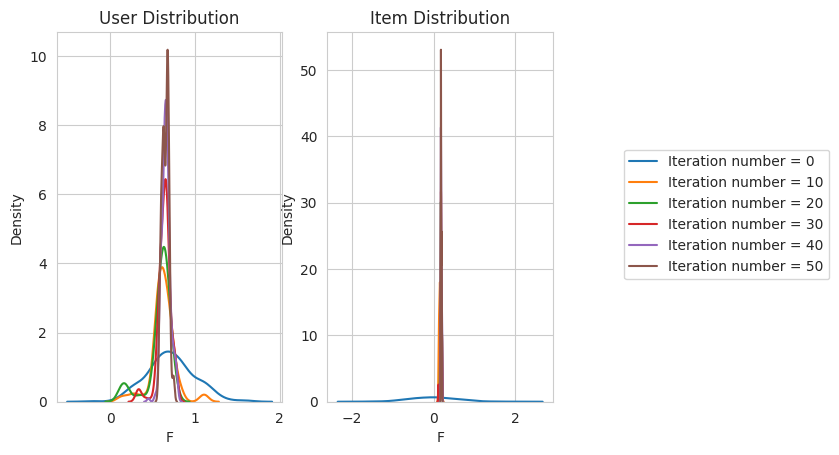
\includegraphics[width=1\textwidth]{images/new_photo/u_1_distr.png}
            \vspace*{-9mm}\caption{$u_{pred}^1$}
        \end{figure}

        \column{0.7\textwidth}
        \begin{figure}
            \centering
            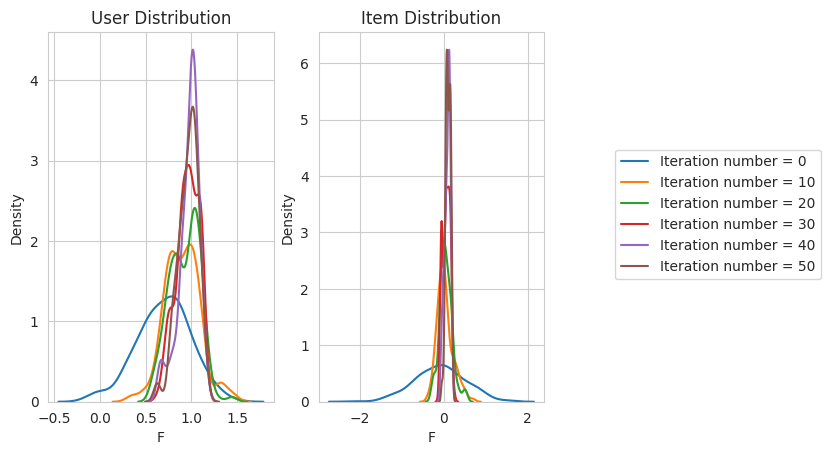
\includegraphics[width=1\textwidth]{images/new_photo/u_2_distr.png}
            \vspace*{-9mm}\caption{$u_{pred}^2$}
        \end{figure}

     \vspace*{-12mm}\end{columns}
        \begin{columns}[c]

        \column{0.7\textwidth}
        \begin{figure}
            \centering
            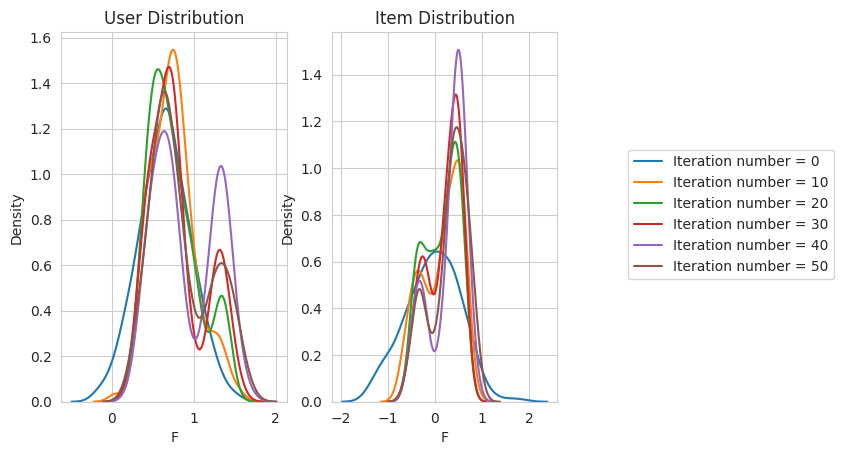
\includegraphics[width=1\textwidth]{images/new_photo/random_distr.png}
             \vspace*{-9mm}\caption{random}
        \end{figure}

        \column{0.7\textwidth}
        \begin{figure}
            \centering
            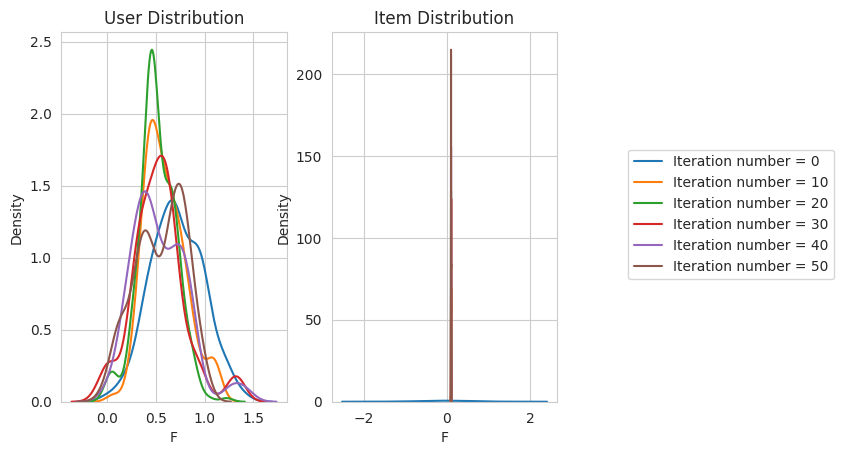
\includegraphics[width=1\textwidth]{images/new_photo/oracle_distr.png}
             \vspace*{-9mm}\caption{oracle}
        \end{figure}

    \end{columns}
\end{frame}


\begin{frame}
    Изменение дисперсий пользователей и товаров со временем
    \begin{columns}[c]
        \column{0.5\textwidth}
        \begin{figure}
            \centering
            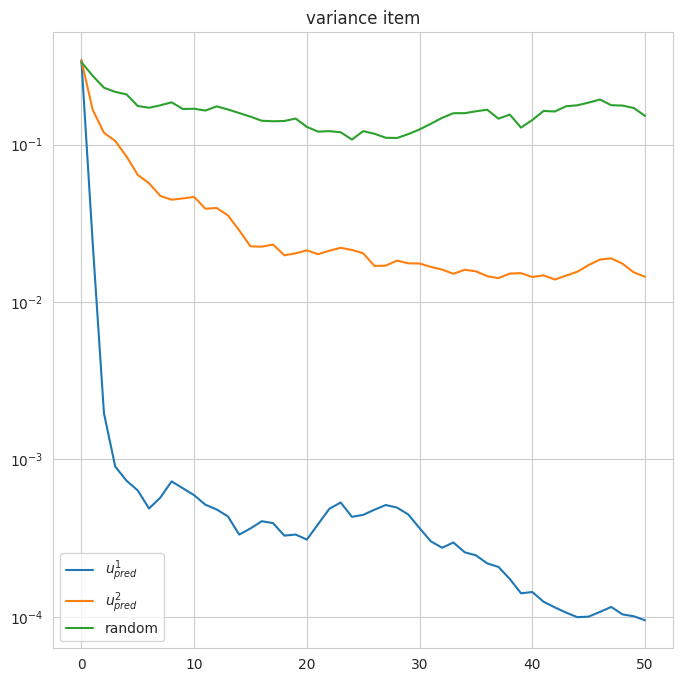
\includegraphics[width=1\textwidth]{images/new_photo/variance_item.png}
            \caption{товары}
        \end{figure}

        \column{0.5\textwidth}
        \begin{figure}
            \centering
            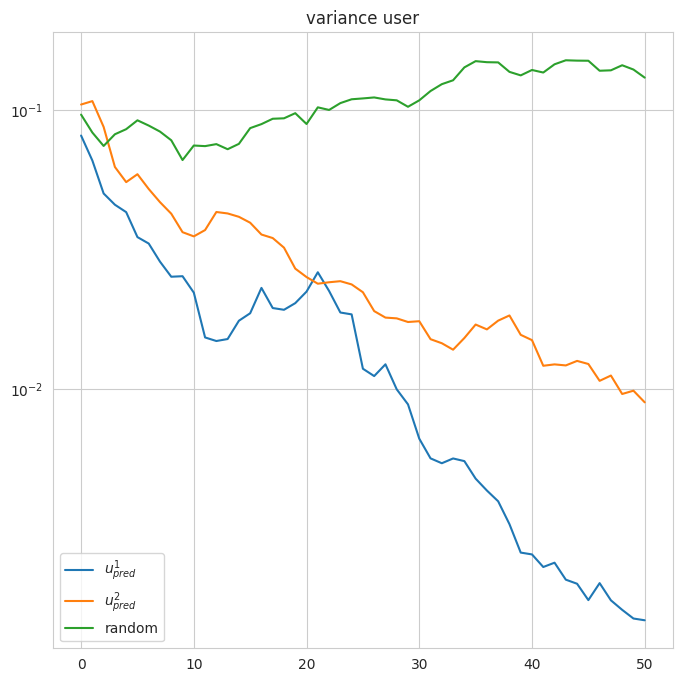
\includegraphics[width=1\textwidth]{images/new_photo/variance_user.png}
            \caption{пользователи}
        \end{figure}
    \end{columns}
    
\end{frame}


\begin{frame}
    \begin{columns}[c]
    
        \column{0.5\textwidth}
        \begin{figure}
            \centering
            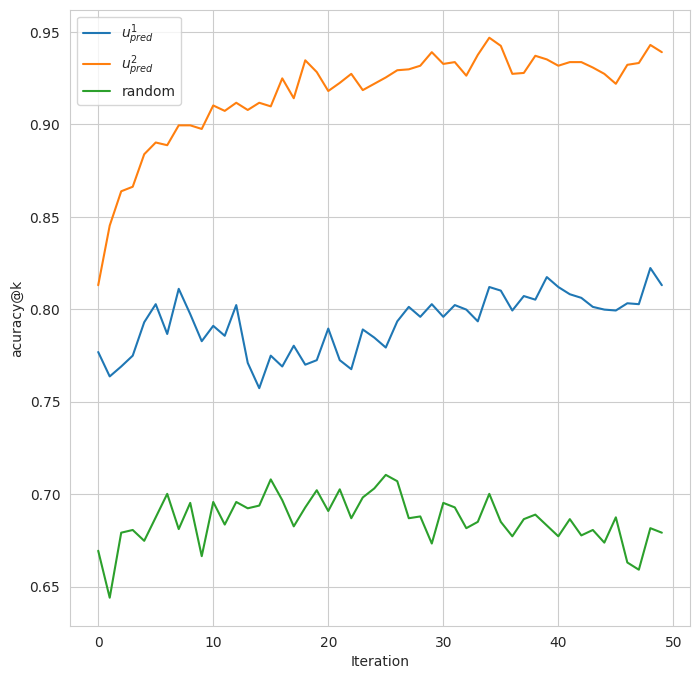
\includegraphics[width=0.7\textwidth]{images/new_photo/accuracy.png}
            \caption{Значение accuracy@8}
        \end{figure}

        \column{0.5\textwidth}
        \begin{figure}
            \centering
            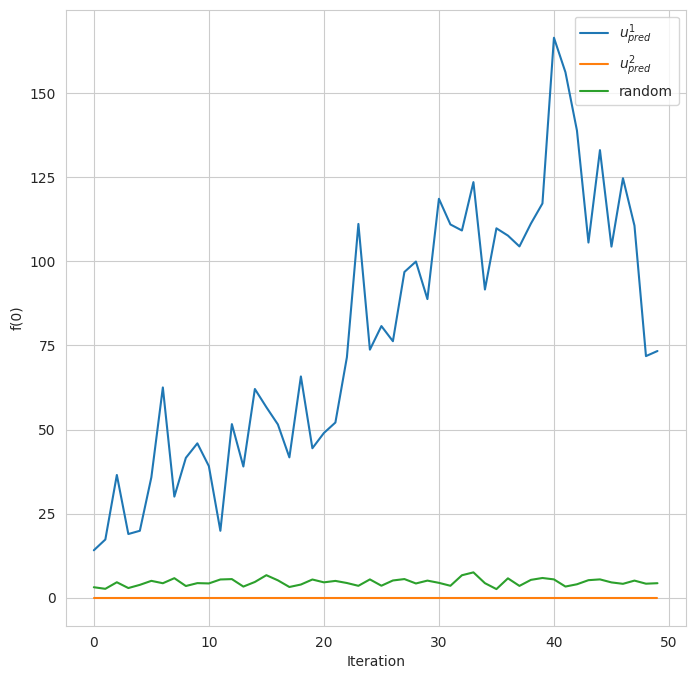
\includegraphics[width=0.7\textwidth]{images/new_photo/f.png}
            \caption{Значение распределения невязок в точке 0}
        \end{figure}

    \end{columns}
    

        \vspace*{-5mm}\begin{figure}
            \centering
            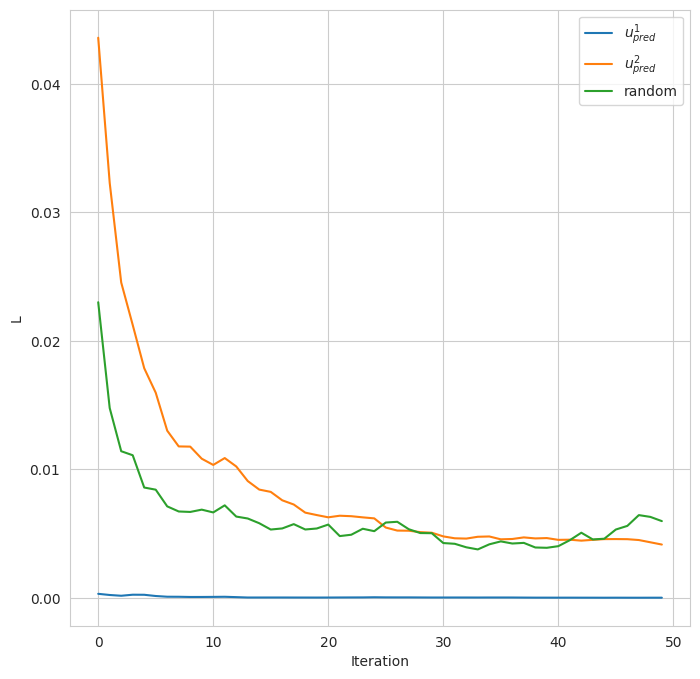
\includegraphics[width=0.4\textwidth]{images/new_photo/L.png}
            \caption{Значение функционала L}
        \end{figure}

    
\end{frame}





%----------------------------------------------------------------------------------------------------------


\begin{frame}{Заключение}
\begin{itemize}
    \item Построена математическая модель динамической во времени рекомендательной системы.  
    \item Для определенного вида алгоримтов удалось найти вид множества вырождения пользователей-товаров.
    \item Предложены гипотезы о вырождениях распределений в зависимости от алгоритма рекомендации.
    \item Проведен вычислительный эксперимент на синтетических данных, который подтвердил теоретические результаты.

\end{itemize}


    
\end{frame}

%----------------------------------------------------------------------------------------------------------

%-----------------------------------------------------------------------------------------------------

\begin{frame}{Публикации по теме}
    \begin{itemize}
    
    \item $[1]$ A. S. Vepricov, A. S. Khritankov. On the problem of repeated supervised learning \url{https://github.com/intsystems/2023-Project-119/blob/master/paper/M1P.pdf}.

    \item $[2]$ Anton Khritankov. Positive feedback loops lead to concept drift in machine learning systems.


    \item $[3]$ Jiang, Ray & Chiappa, Silvia & Lattimore, Tor & György, András & Kohli, Pushmeet. (2019). Degenerate Feedback Loops in Recommender Systems
  
    \end{itemize}
\end{frame}


\end{document} 